%10
\begin{frame}
  \begin{itemize}
    \item Egyszerű szövegfájl (jellemzően UTF-8 kódolással)
    \item Dokumentum \emph{strukturájának} jelölésére, pl.
    \begin{itemize}
      \item fejlécek
      \item listák
      \item bekezdések
      \item hiperhivatkozások
    \end{itemize}
    \item Megjelenítést befolyásolja
    \begin{itemize}
      \item böngésző alapértelmezése
      \item felhasználó globális beállításai a böngészőben
      \item stíluslapok (CSS)
    \end{itemize}
    \item Megjelenítés leválasztása
    \begin{itemize}
      \item helyes megjelenítés többféle böngészőben
      \item könnyebben karbantartható oldalak
      \item nem vizuális böngészők támogatása
    \end{itemize}
  \end{itemize}
\end{frame}

%11
\begin{frame}
  \begin{itemize}
    \item Struktúra kialakítása az SGML-hez hasonlóan: egymásba ágyazható elemek, címkék, attribútumok
    \item Beágyazási szabályok, használható attribútumok $\to$ ,,szabvány'' (ajánlás)
    \item Helytelenül formázott dokumentumok
    \begin{itemize}
      \item Nincsenek hibaüzenetek
      \item A böngésző a tőle telhető legjobb eredményt nyújtja
      \item Kompatibilitási okokból az elavult megoldásokat is kénytelen támogatni
      \item Ellenőrzés különböző böngészőkben vs. \hiv{\href{https://validator.w3.org/}{szintaxis validálás}}
    \end{itemize}
  \end{itemize}
\end{frame}

%12
\begin{frame}
  \scriptsize
  \begin{exampleblock}{\textattachfile{hibas.html}{hibas.html}}
    \lstinputlisting[language=HTML]{hibas.html}
  \end{exampleblock}
  \begin{columns}[T]
    \column{0.3\textwidth}
      \begin{center}
        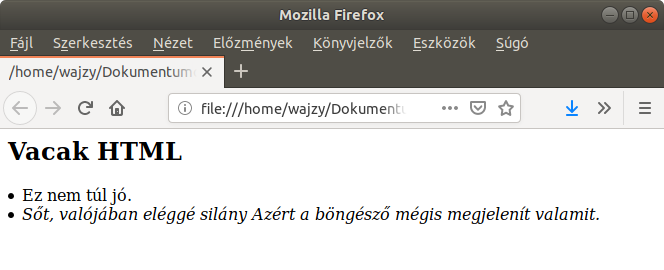
\includegraphics[width=\textwidth]{hibas_firefox.png} \\
        Mozilla Firefox 69.0
      \end{center}
    \column{0.3\textwidth}
      \begin{center}
        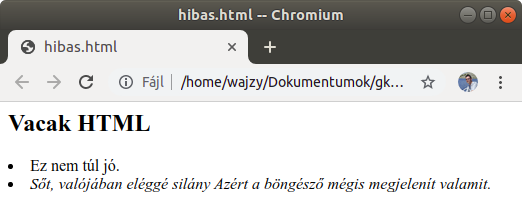
\includegraphics[width=\textwidth]{hibas_chromium.png} \\
        Chromium 76.0.3809.100
      \end{center}
    \column{0.3\textwidth}
      \begin{center}
        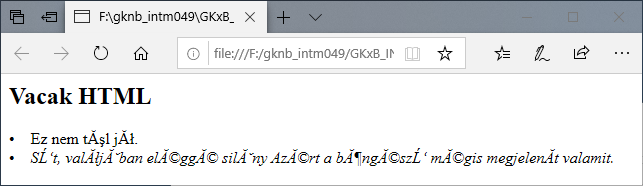
\includegraphics[width=\textwidth]{hibas_edge.png} \\
        Microsoft Edge 44.17763.1.0
      \end{center}
  \end{columns}
\end{frame}
